\section{Link Layer}

\subsection{Introduction and services}

\key{Link Layer Services}
\begin{figure}[H]
  \centering
  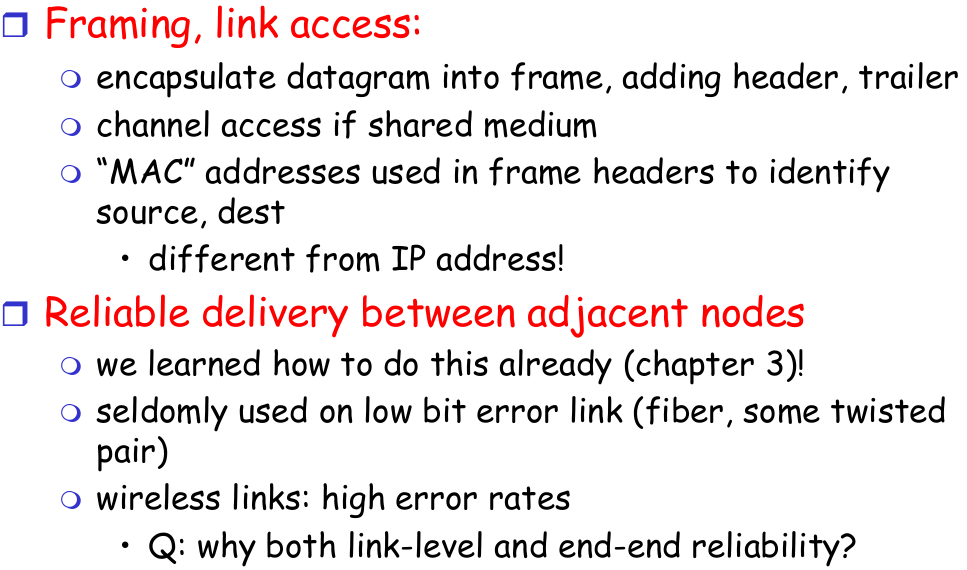
\includegraphics[width=0.48\textwidth]{link_services1}
  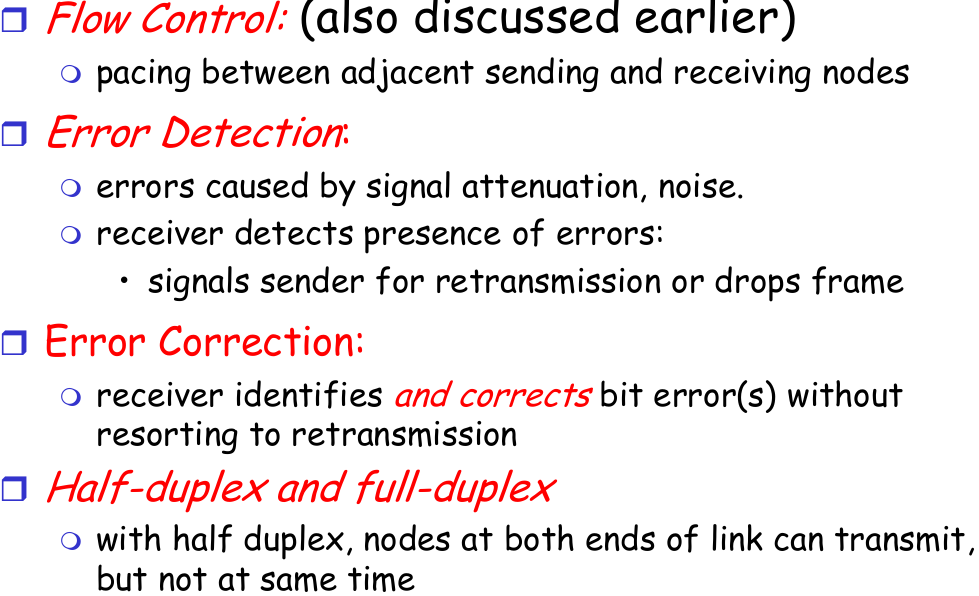
\includegraphics[width=0.48\textwidth]{link_services2}
\end{figure}

\subsection{Error detection and correction}

\key{Hamming distance} The (min) number of bits that differ, that is, need to
be flipped/inverted to change from one codeword to the other.

If the minimum Hamming distance between any two valid codewords is $d$ , then
detect any error up to $d-1$ bits, and can correct any error up to $(d-1)/2$ (if
$d$ is odd), or $d/2-1$ (if $d$ is even) bits.

\key{Checksumming: Cyclic Redundancy Check}
\begin{figure}[H]
  \centering
  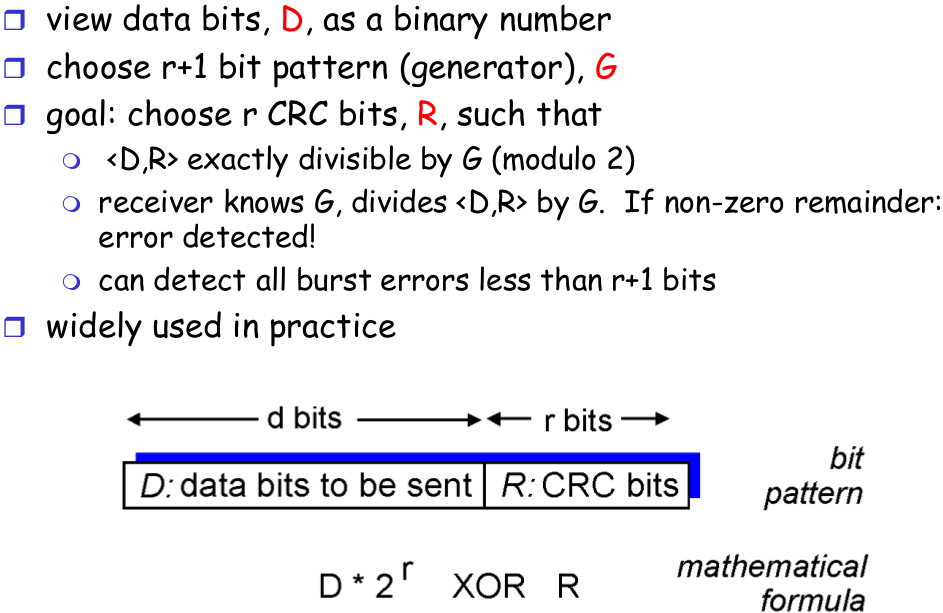
\includegraphics[width=0.48\textwidth]{crc}
  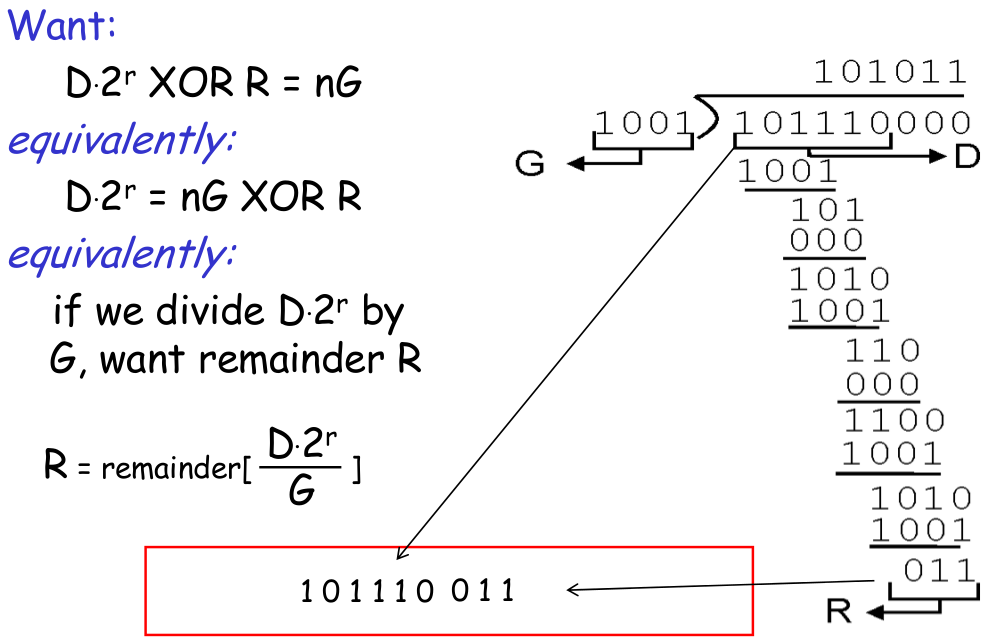
\includegraphics[width=0.48\textwidth]{crc_example}
\end{figure}

\subsection{Multiple access protocols}

\key{MAC Protocols: a taxonomy}
\begin{figure}[H]
  \centering
  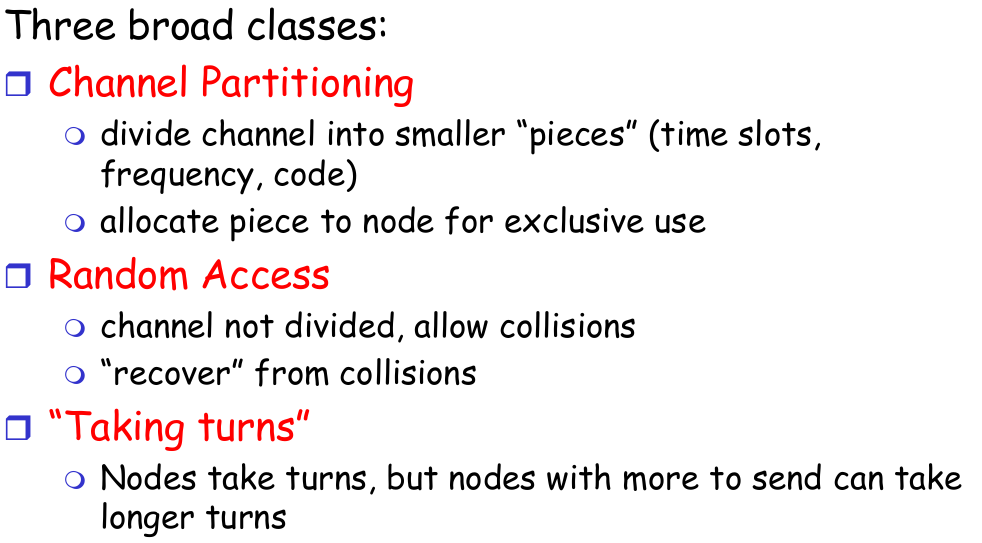
\includegraphics[width=0.48\textwidth]{mac}
\end{figure}

\key{Slotted ALOHA}
\begin{figure}[H]
  \centering
  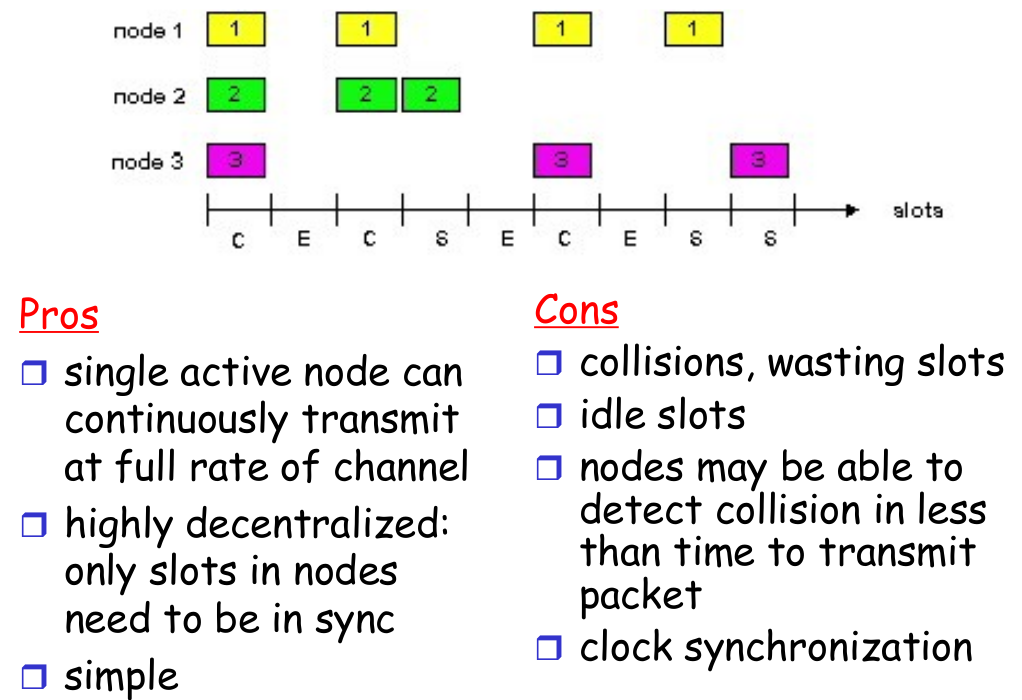
\includegraphics[width=0.48\textwidth]{slotted_aloha}
  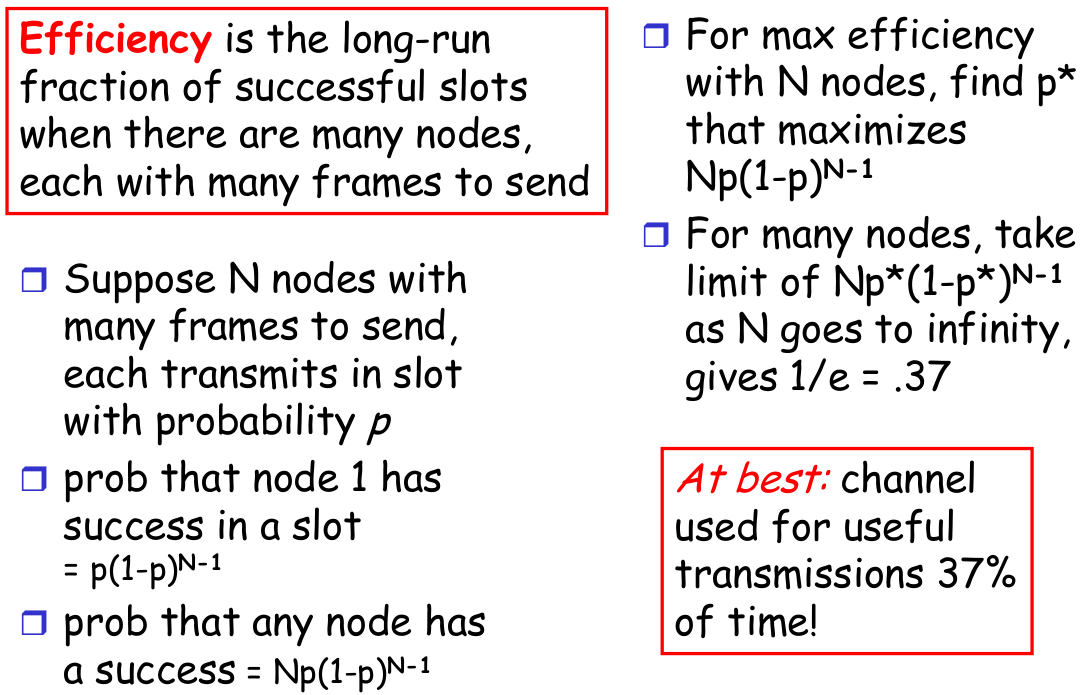
\includegraphics[width=0.48\textwidth]{slotted_aloha_p}
\end{figure}

\key{Pure (unslotted) ALOHA}
\begin{figure}[H]
  \centering
  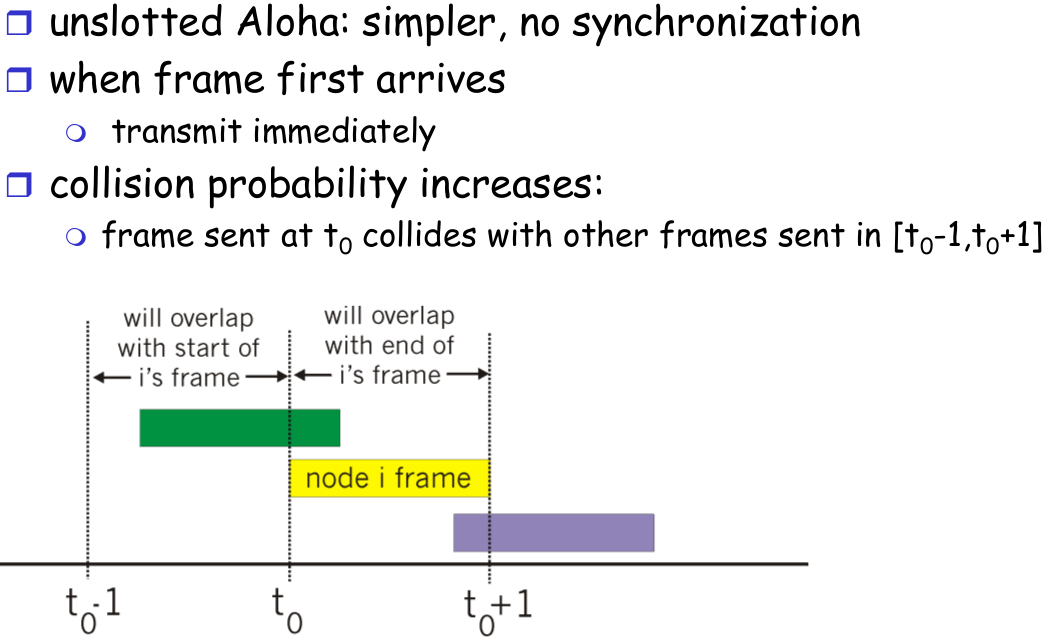
\includegraphics[width=0.48\textwidth]{pure_aloha}
  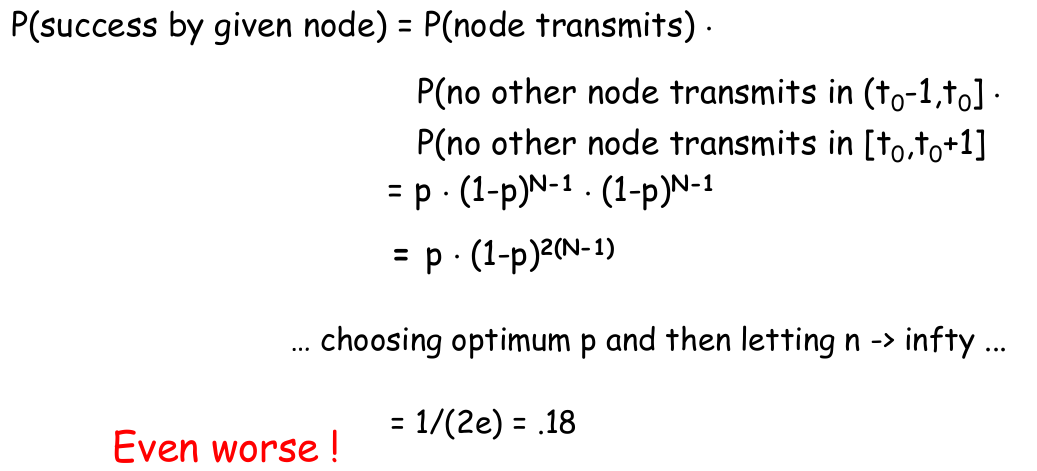
\includegraphics[width=0.48\textwidth]{pure_aloha_p}
\end{figure}

\key{CSMA (Carrier Sense Multiple Access)}
\begin{figure}[H]
  \centering
  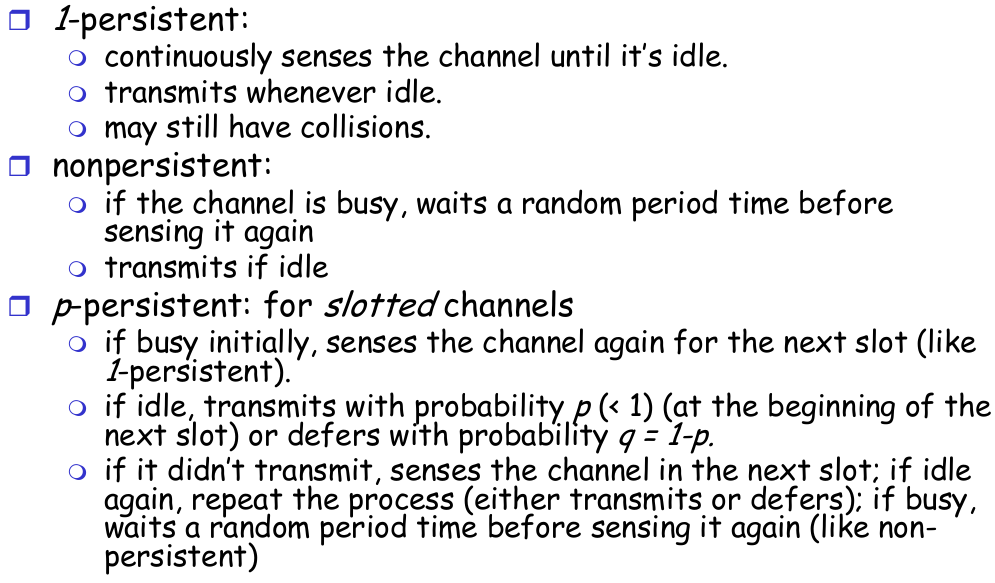
\includegraphics[width=0.48\textwidth]{csma1}
  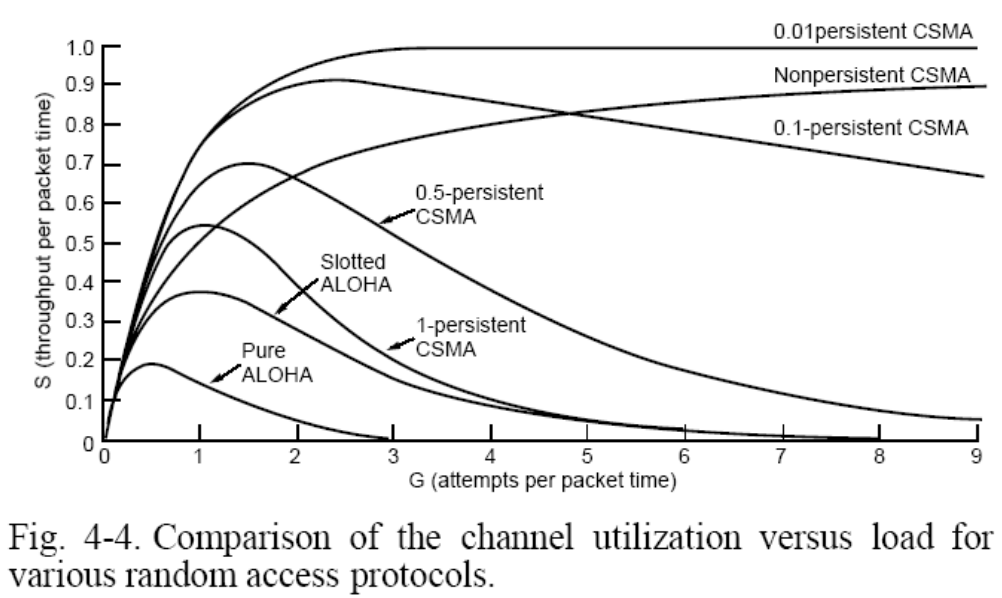
\includegraphics[width=0.48\textwidth]{csma2}
\end{figure}

\key{CSMA/CD Collision Detection Delay}
\begin{figure}[H]
  \centering
  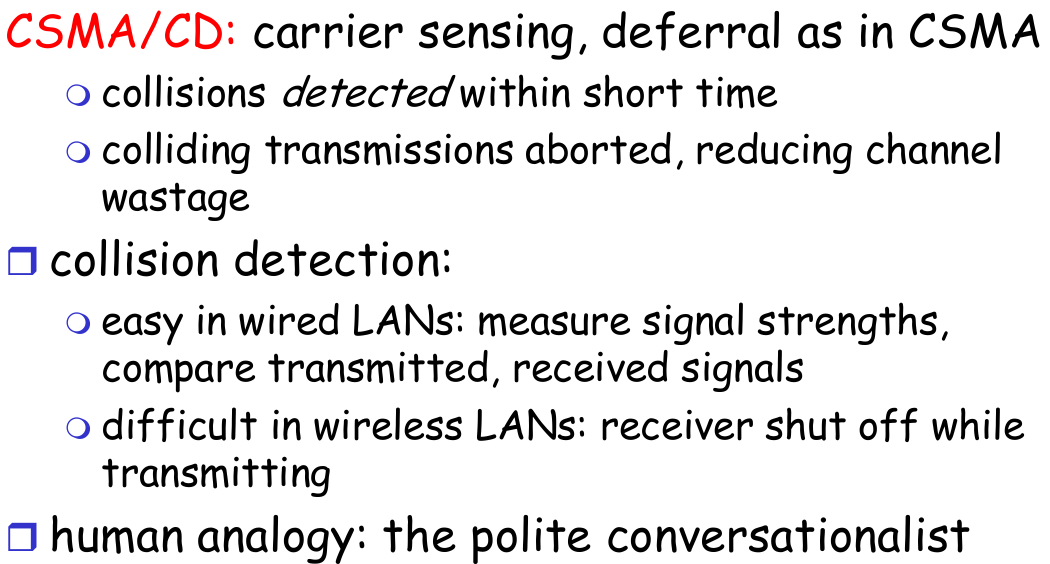
\includegraphics[width=0.48\textwidth]{csma_cd}
  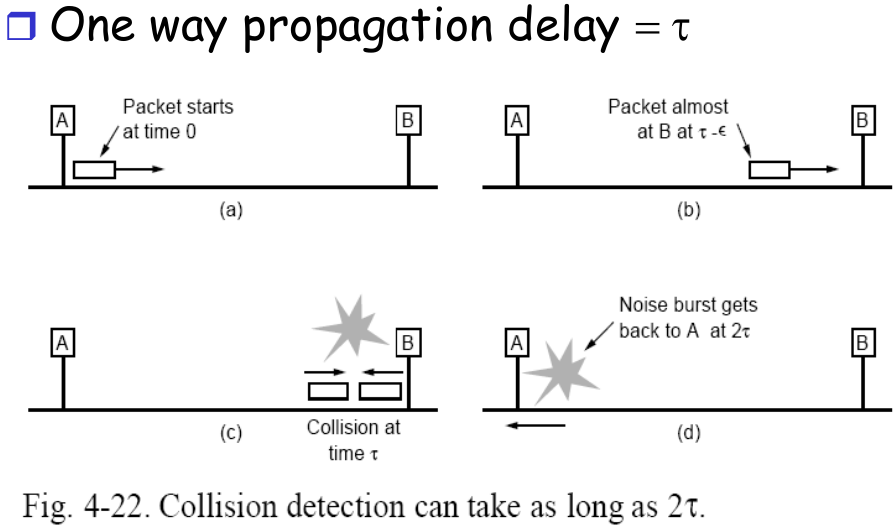
\includegraphics[width=0.48\textwidth]{csma_cd_delay}
\end{figure}

\key{Taking Turns MAC protocols}
\begin{figure}[H]
  \centering
  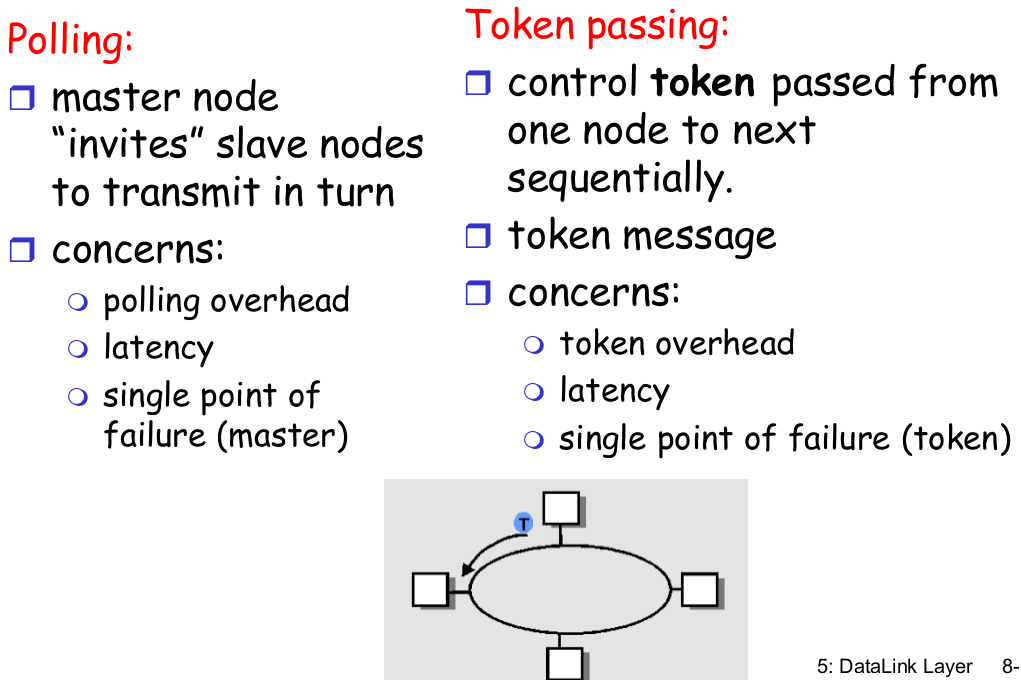
\includegraphics[width=0.48\textwidth]{take_turns}
  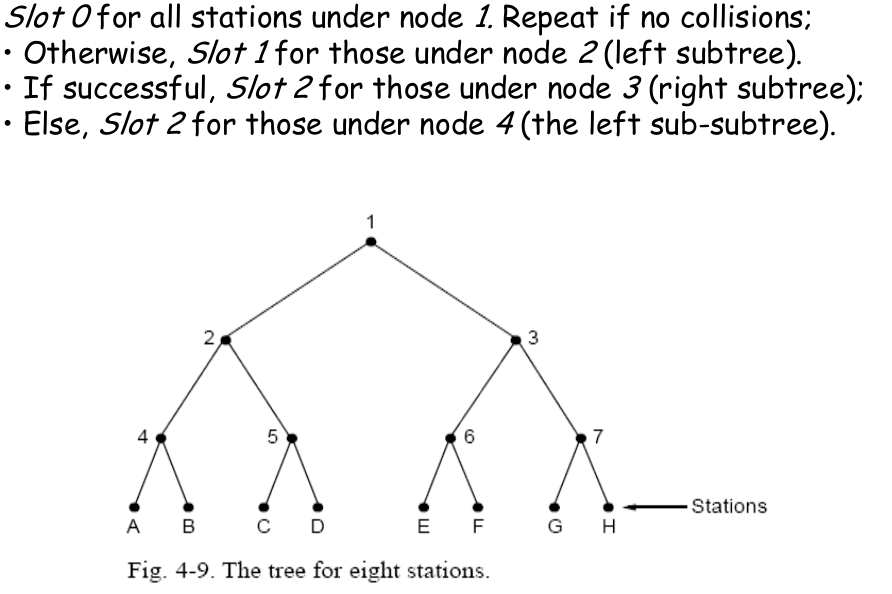
\includegraphics[width=0.48\textwidth]{adaptive_tree}
\end{figure}

\subsection{Link-Layer Addressing}


\key{MAC (or LAN or physical or Ethernet) address} used to get datagram from one interface to
another physically-connected interface (same network)

\key{ARP: Address Resolution Protocol}
\begin{figure}[H]
  \centering
  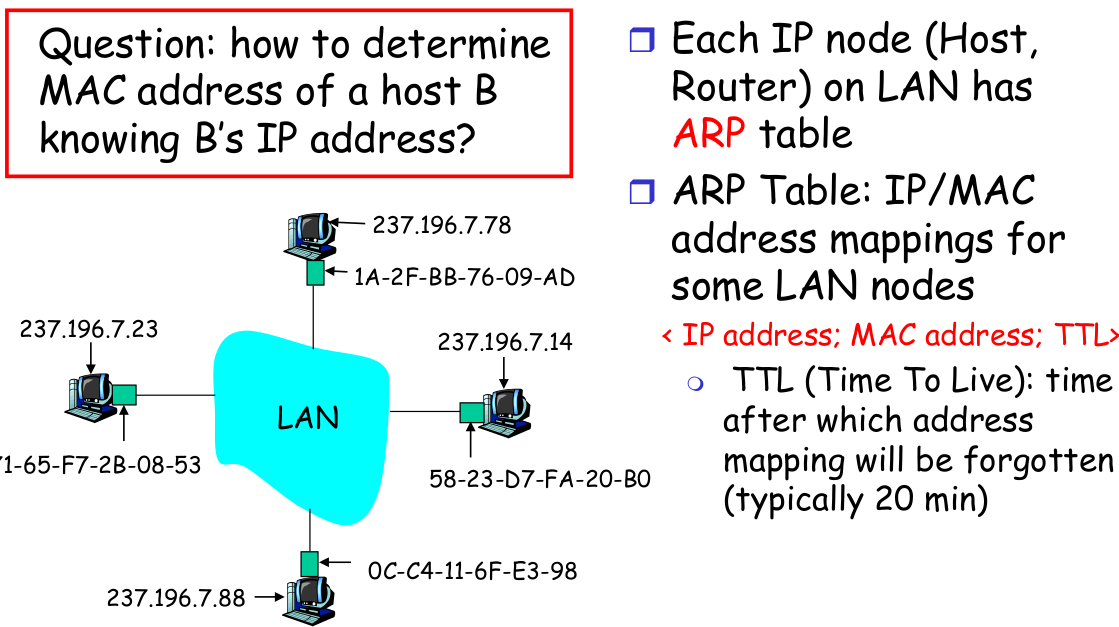
\includegraphics[width=0.48\textwidth]{arp2}
  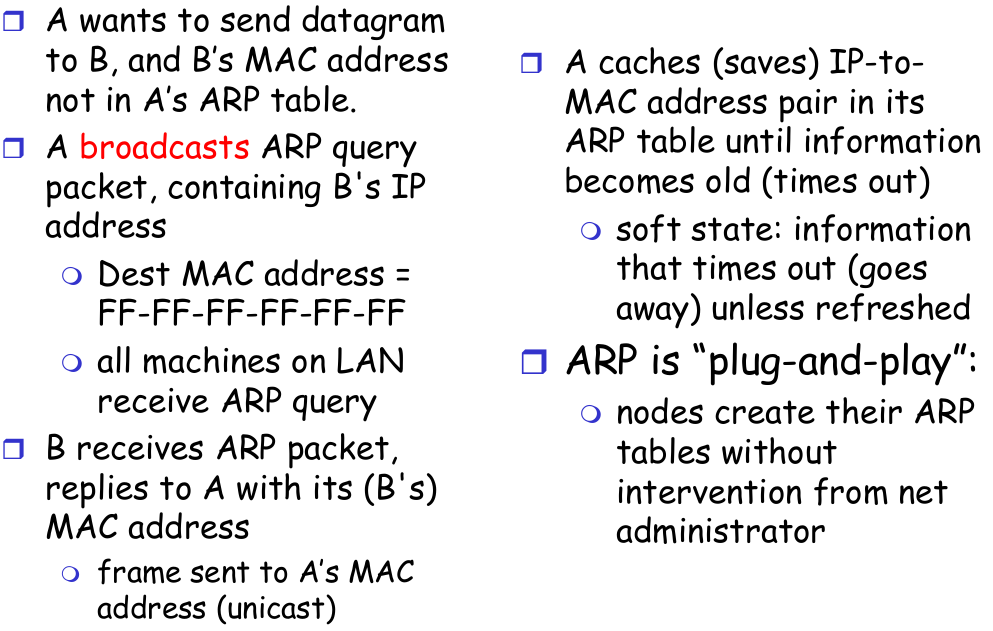
\includegraphics[width=0.48\textwidth]{arp}
\end{figure}

\key{Routing to another LAN}
\begin{figure}[H]
  \centering
  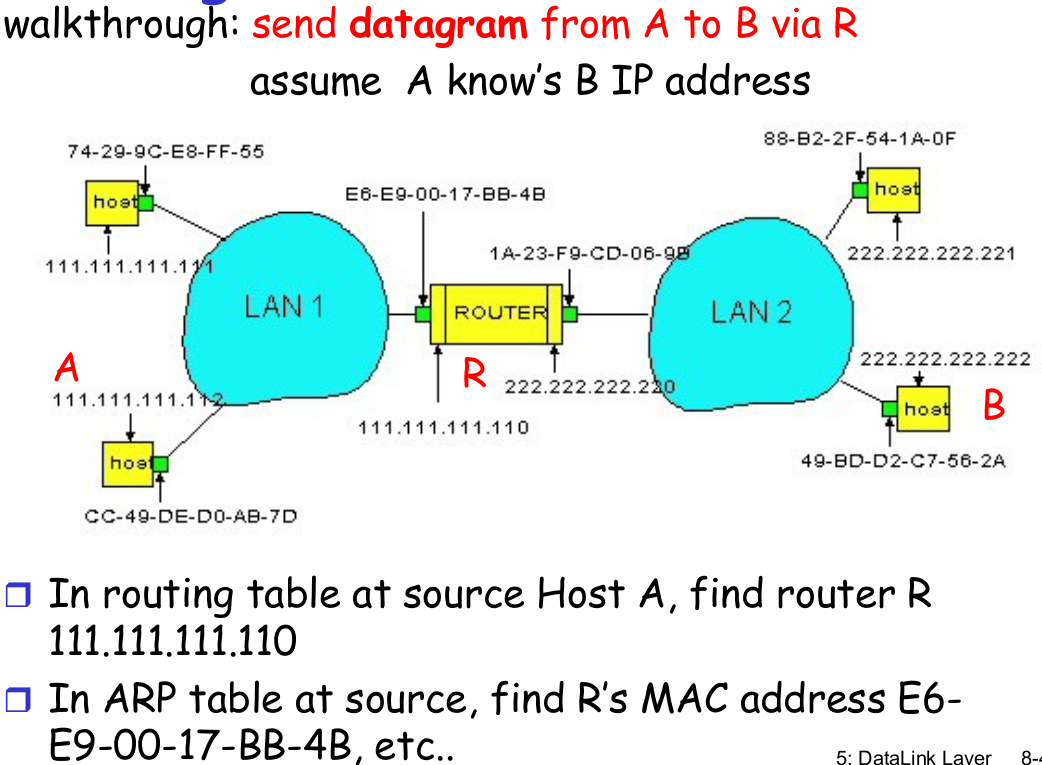
\includegraphics[width=0.48\textwidth]{arp_other_lan}
  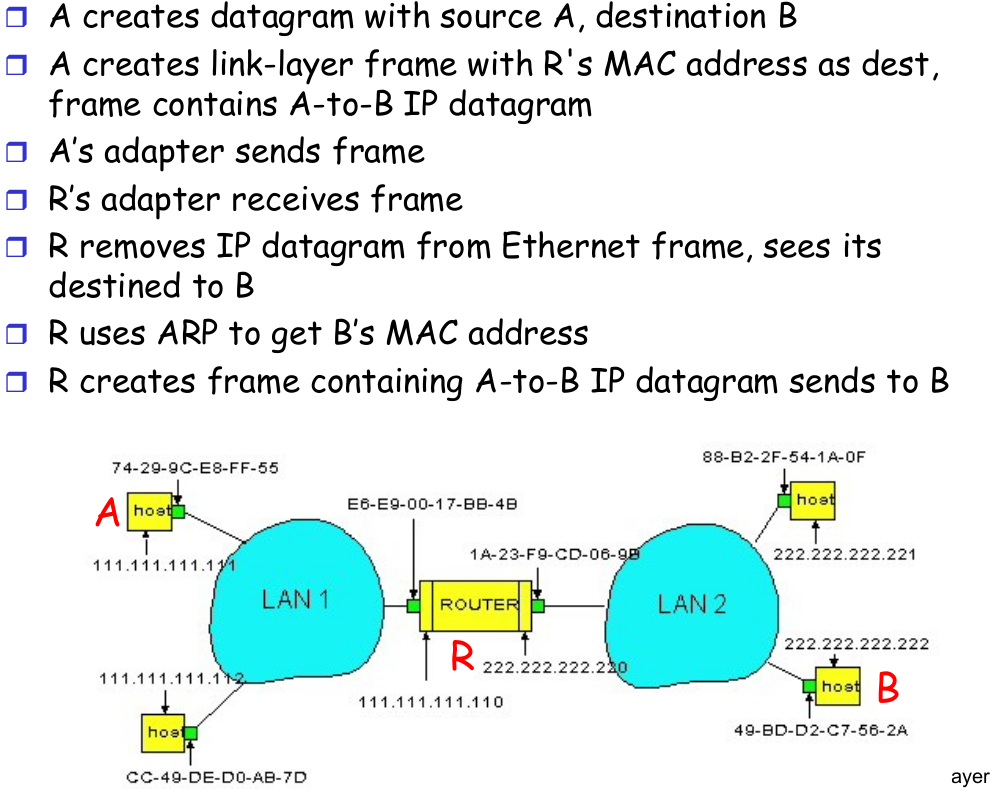
\includegraphics[width=0.48\textwidth]{arp_other_lan2}
\end{figure}

\subsection{Ethernet}

\key{Ethernet Frame Structure}
\begin{figure}[H]
  \centering
  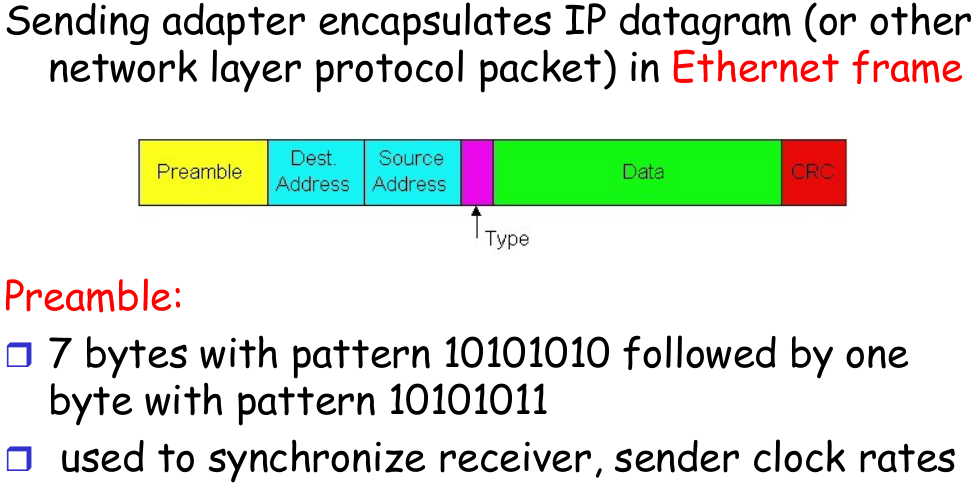
\includegraphics[width=0.48\textwidth]{eth_frame1}
  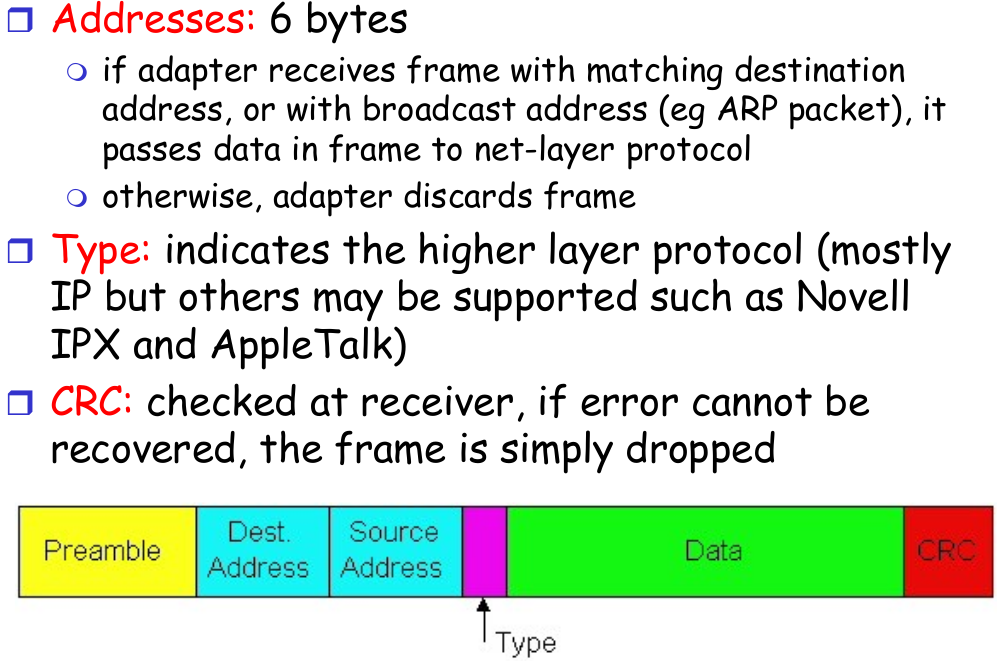
\includegraphics[width=0.48\textwidth]{eth_frame2}
\end{figure}

\key{Ethernet CSMA/CD algorithm}
\begin{figure}[H]
  \centering
  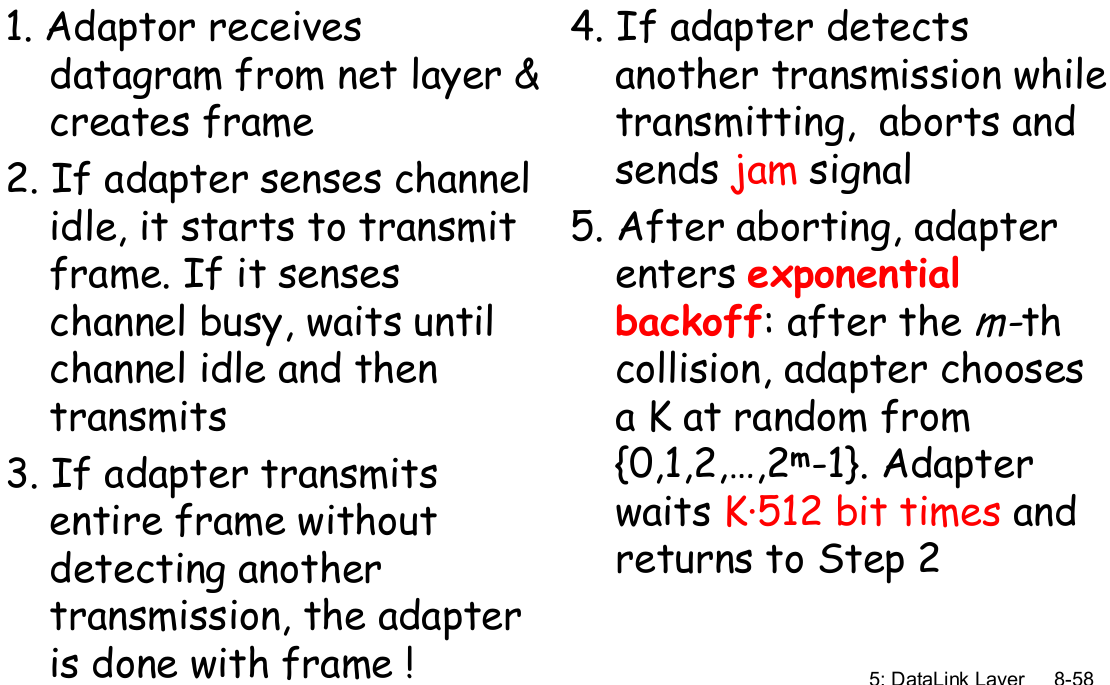
\includegraphics[width=0.48\textwidth]{eth_csma1}
  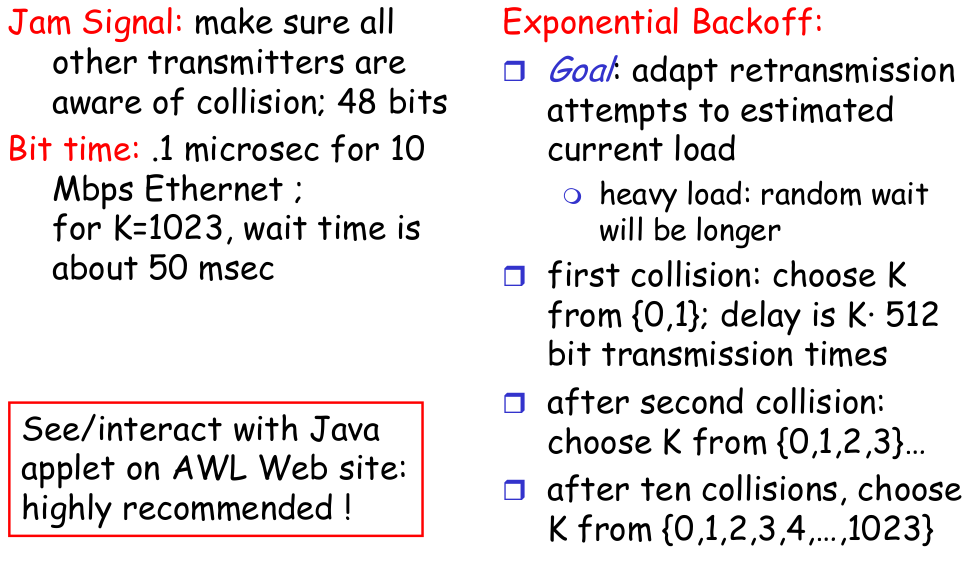
\includegraphics[width=0.48\textwidth]{eth_csma2}
\end{figure}

\key{CSMA/CD efficiency}
\begin{figure}[H]
  \centering
  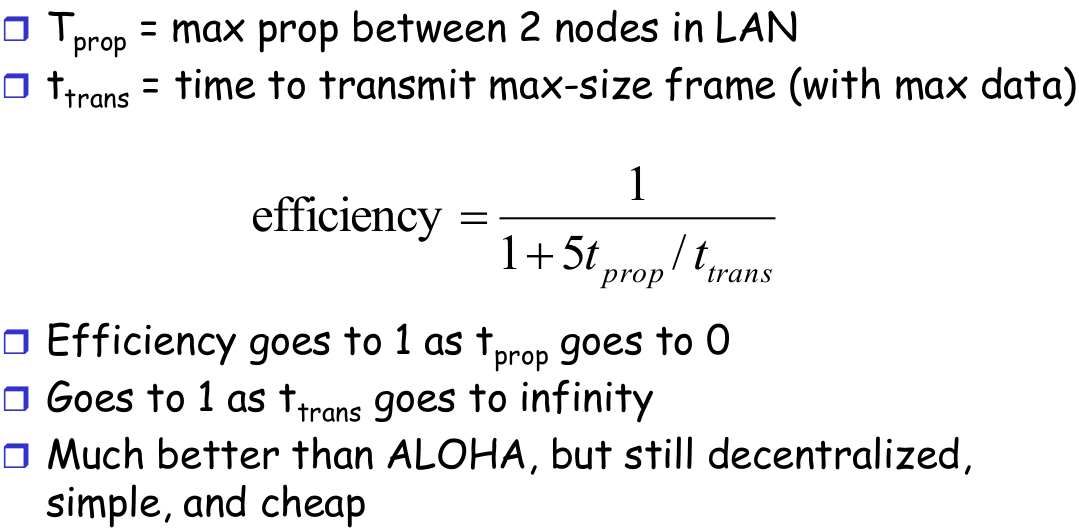
\includegraphics[width=0.48\textwidth]{csma_cd_eff1}
  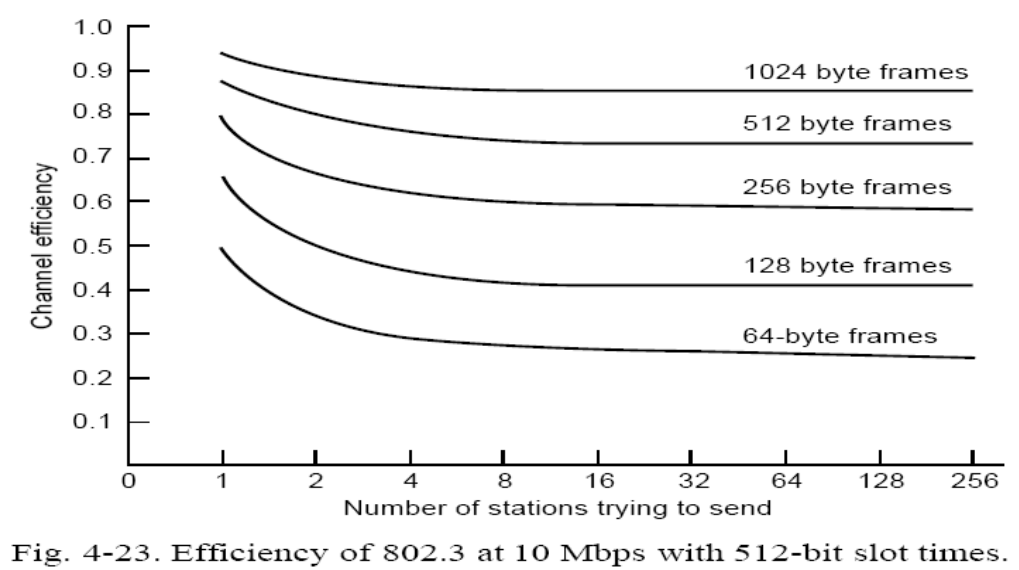
\includegraphics[width=0.48\textwidth]{csma_cd_eff2}
\end{figure}

\key{802.3 Ethernet Standards: Link \& Physical Layers}
\begin{figure}[H]
  \centering
  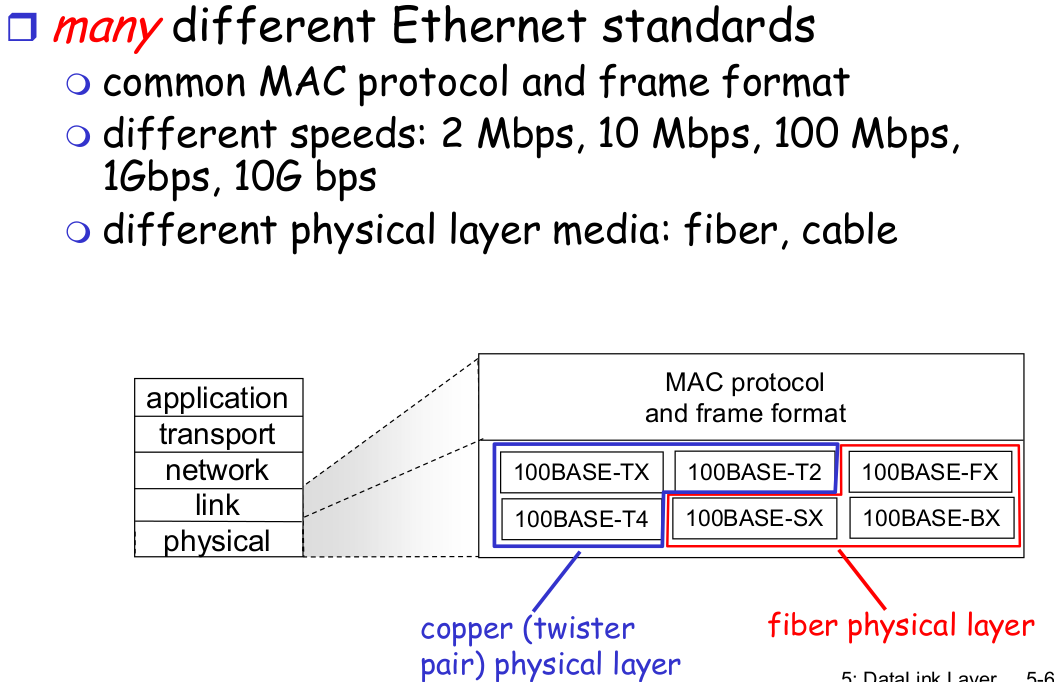
\includegraphics[width=0.48\textwidth]{802_3}
\end{figure}

\subsection{Interconnections: Hubs and switches}

\key{Hubs and Switches}
\begin{figure}[H]
  \centering
  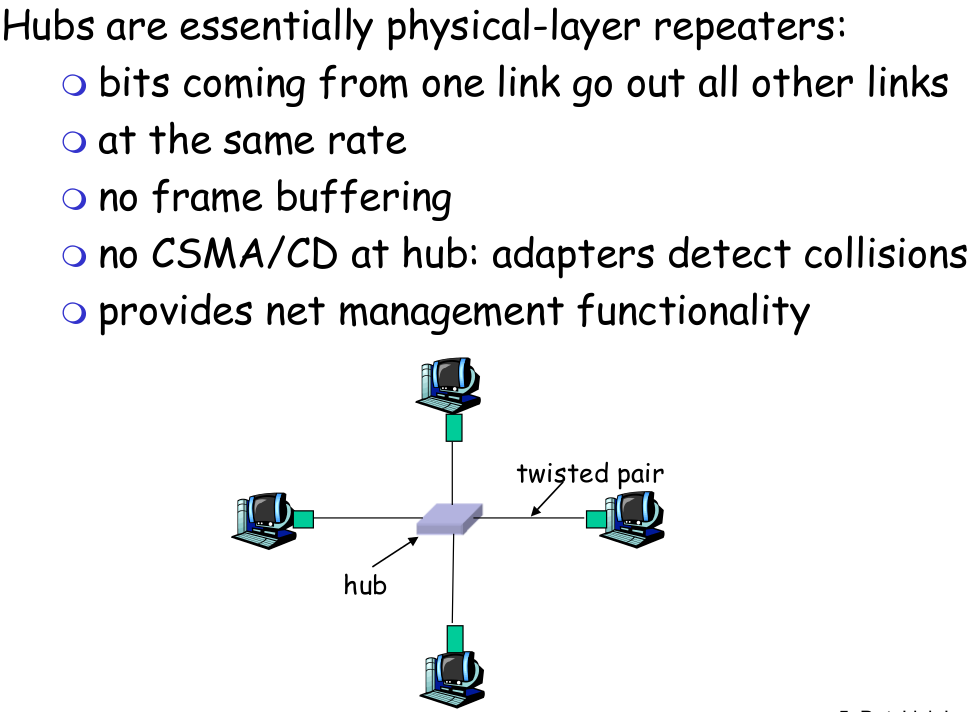
\includegraphics[width=0.48\textwidth]{hub}
  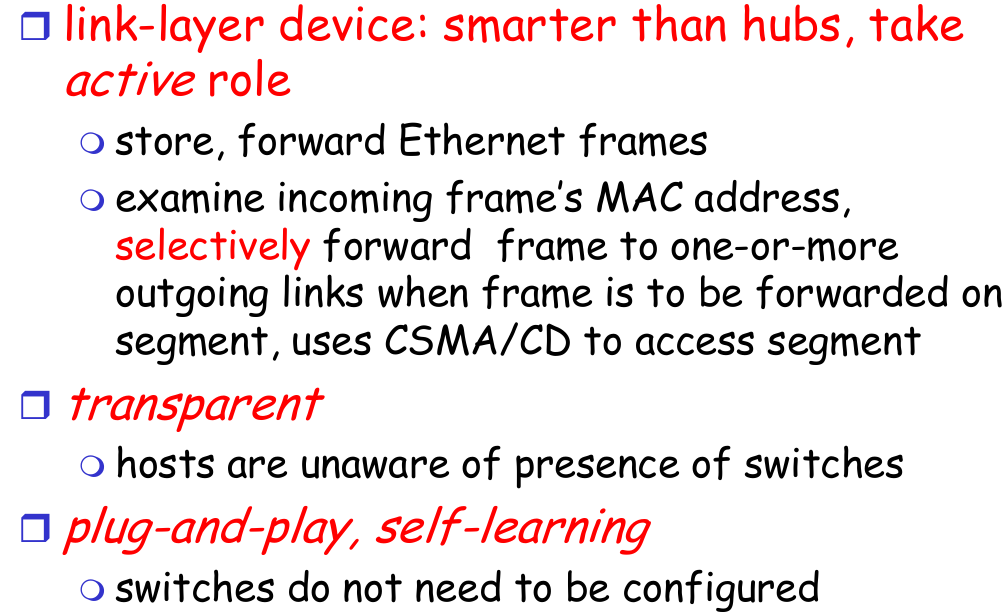
\includegraphics[width=0.48\textwidth]{switch}
\end{figure}

\key{Switch: frame filtering/forwarding}
\begin{figure}[H]
  \centering
  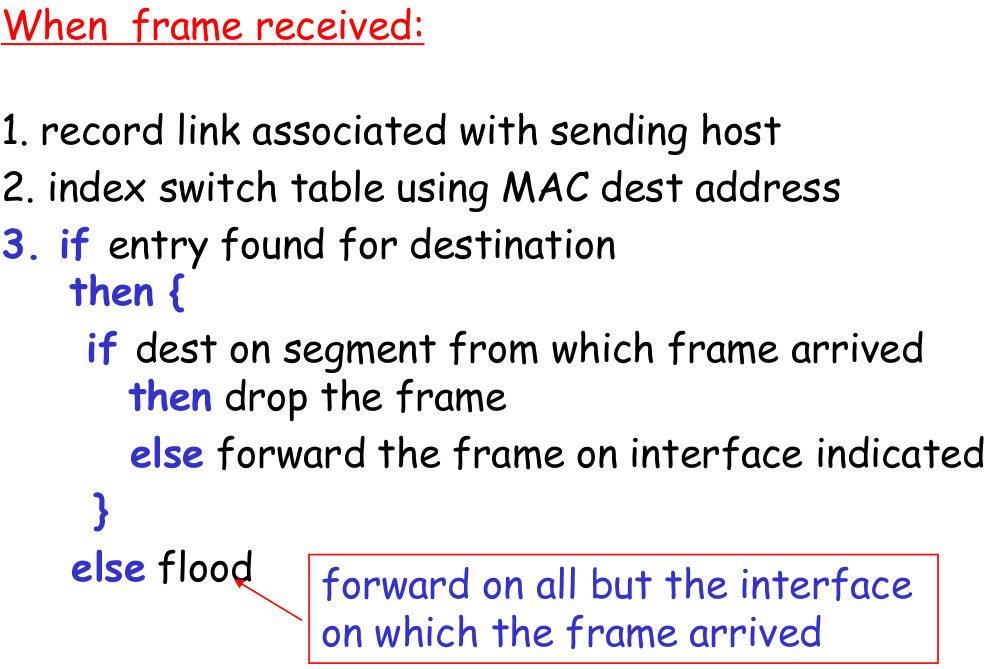
\includegraphics[width=0.48\textwidth]{switch_table}
  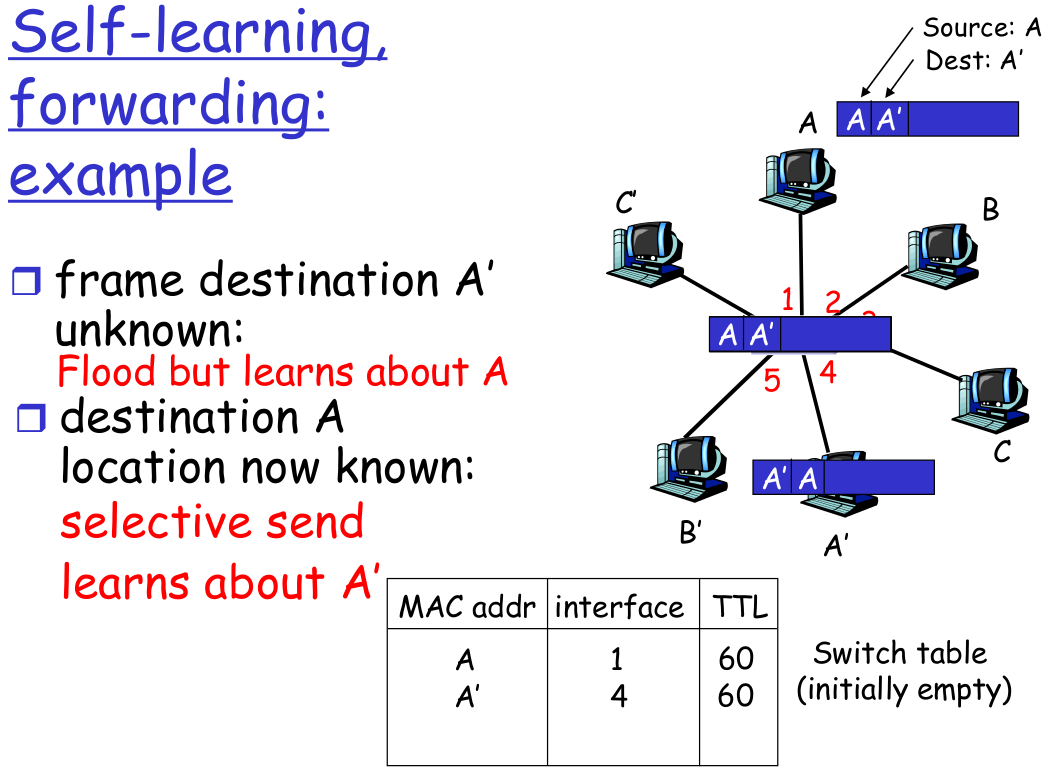
\includegraphics[width=0.48\textwidth]{switch_table2}
\end{figure}

\key{Switches vs. Routers}
\begin{figure}[H]
  \centering
  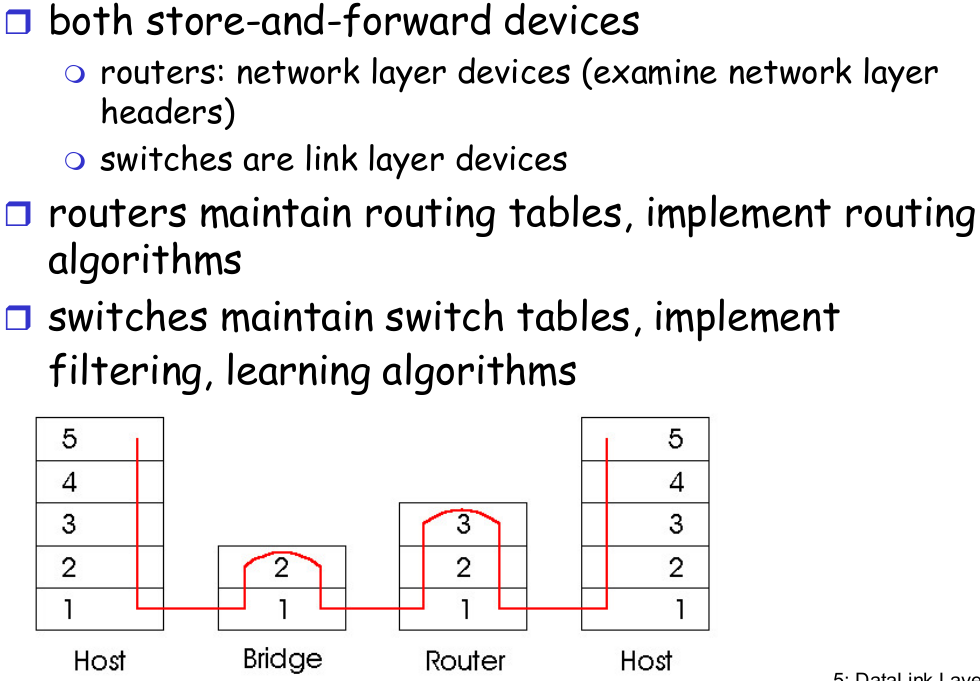
\includegraphics[width=0.48\textwidth]{switch_vs_router}
\end{figure}

\key{VLANs}
\begin{figure}[H]
  \centering
  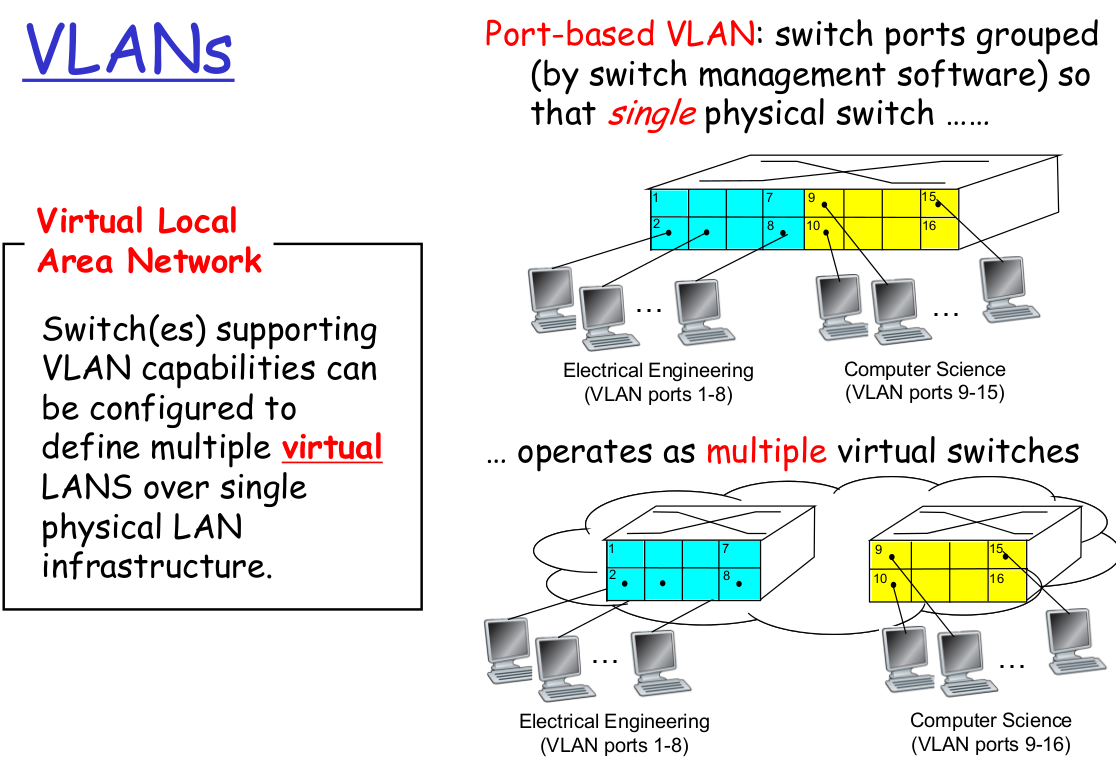
\includegraphics[width=0.48\textwidth]{vlan1}
  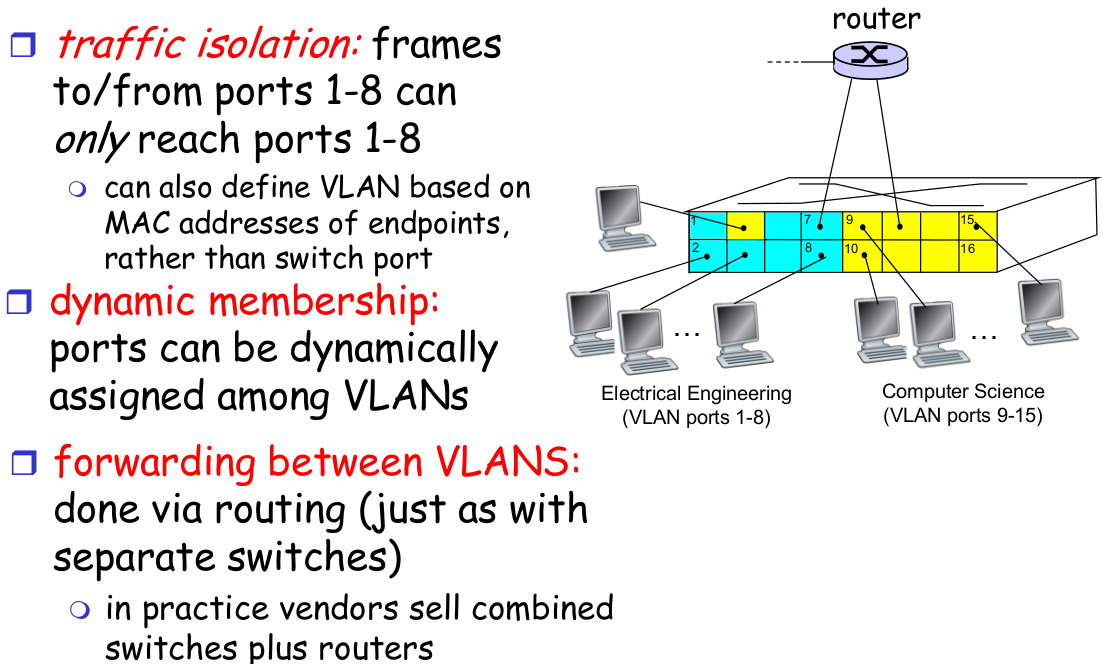
\includegraphics[width=0.48\textwidth]{vlan2}
\end{figure}

\subsection{MPLS}

\key{Multiprotocol label switching (MPLS)}
\begin{figure}[H]
  \centering
  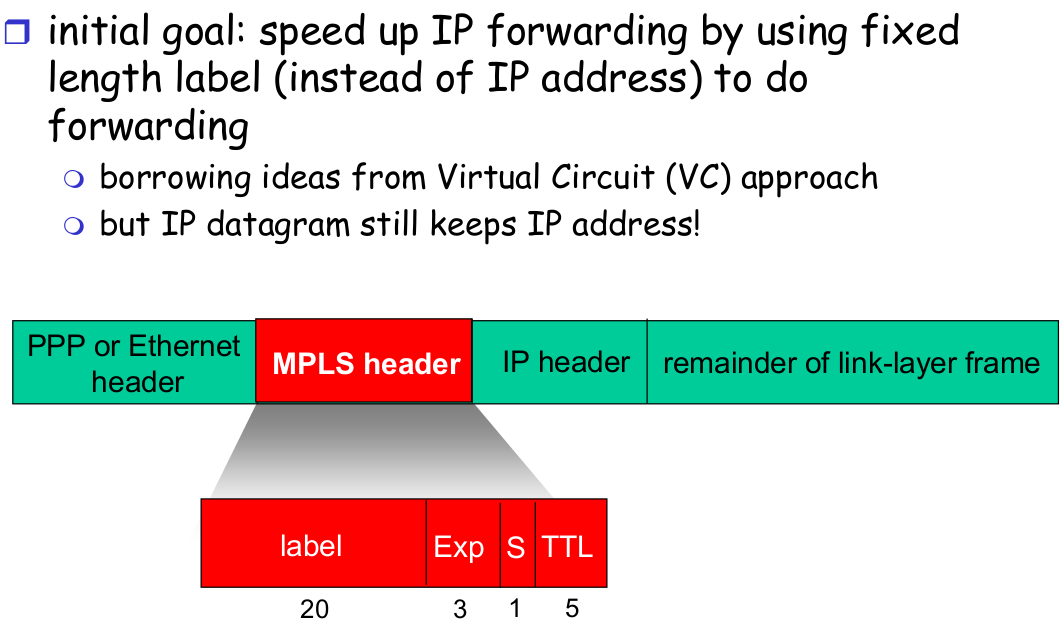
\includegraphics[width=0.48\textwidth]{mpls1}
  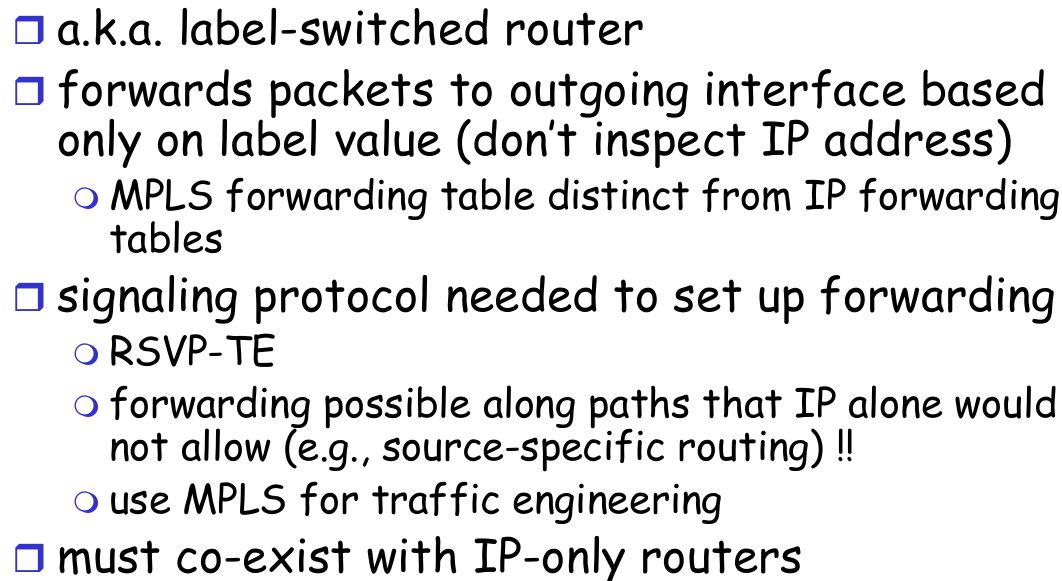
\includegraphics[width=0.48\textwidth]{mpls2}
\end{figure}

\subsection{A day in the life}
\begin{figure}[H]
  \centering
  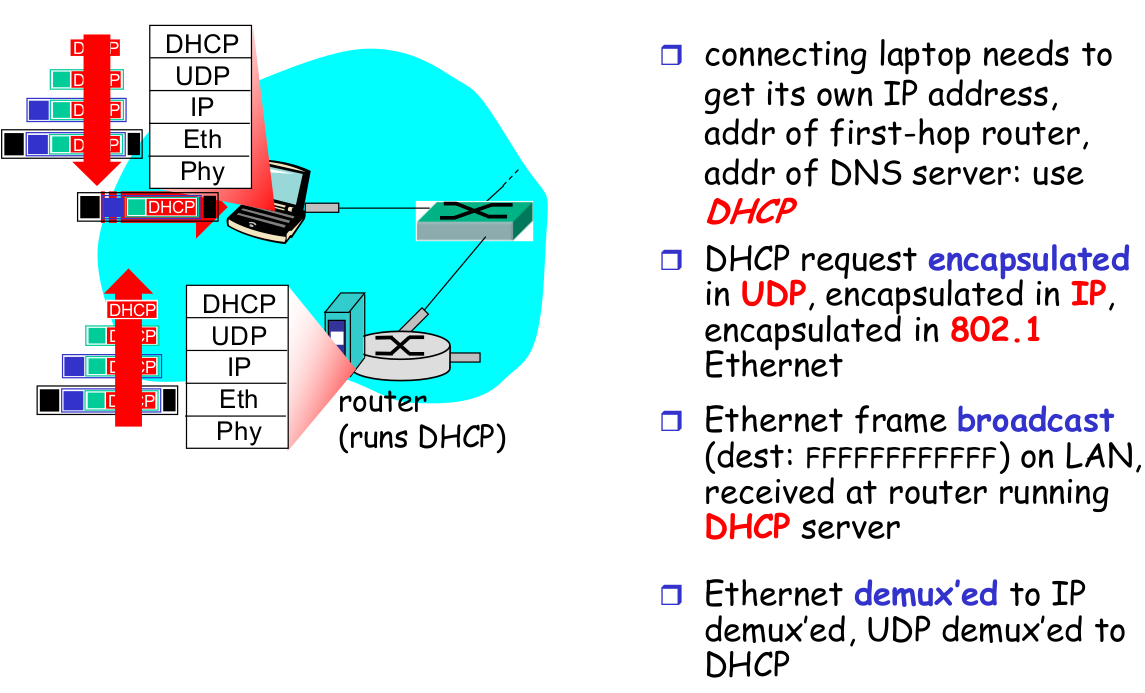
\includegraphics[width=0.48\textwidth]{day1}
  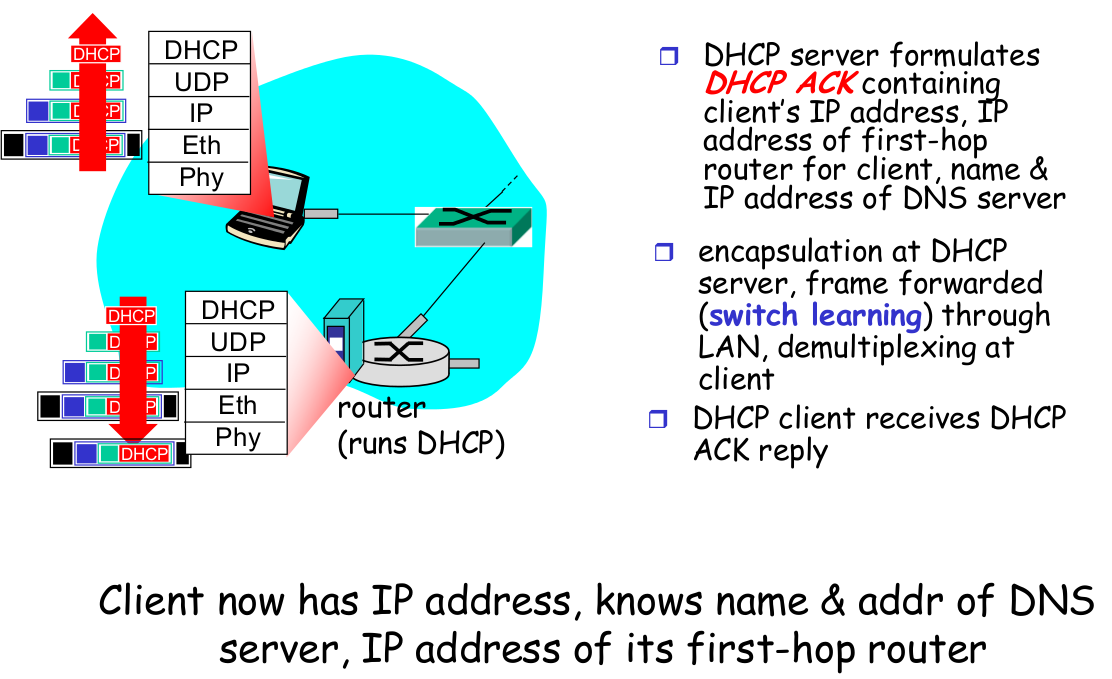
\includegraphics[width=0.48\textwidth]{day2}
  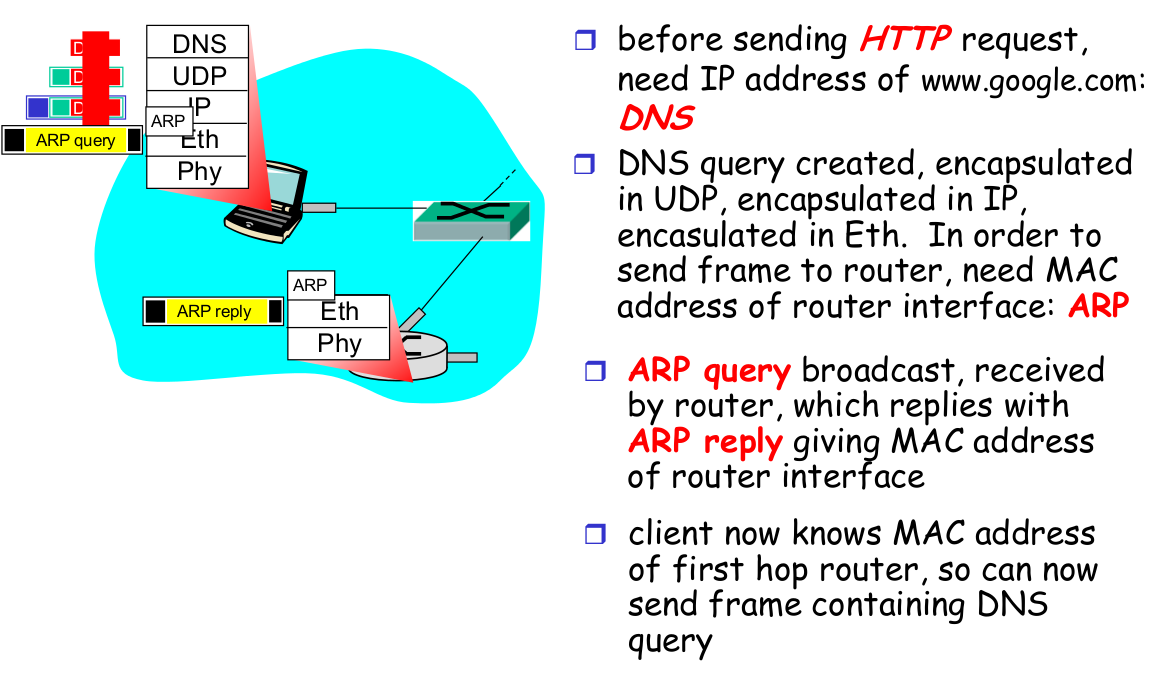
\includegraphics[width=0.48\textwidth]{day3}
  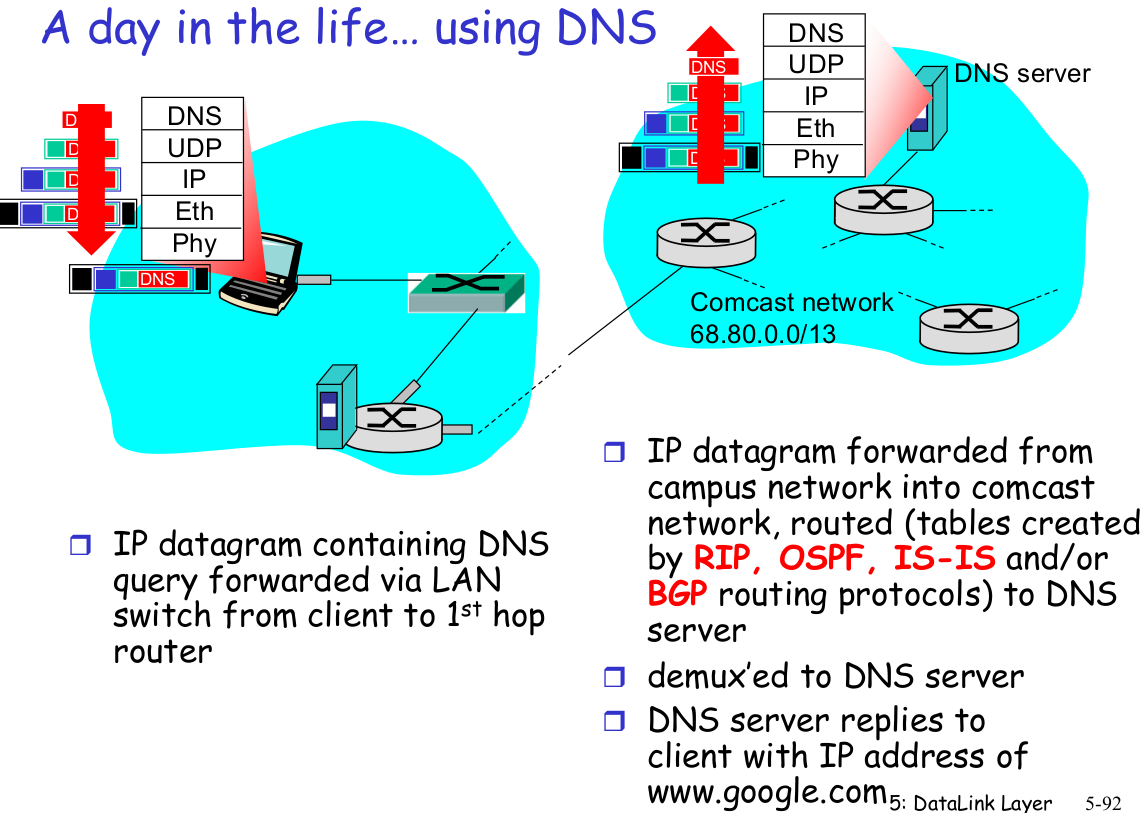
\includegraphics[width=0.48\textwidth]{day4}
  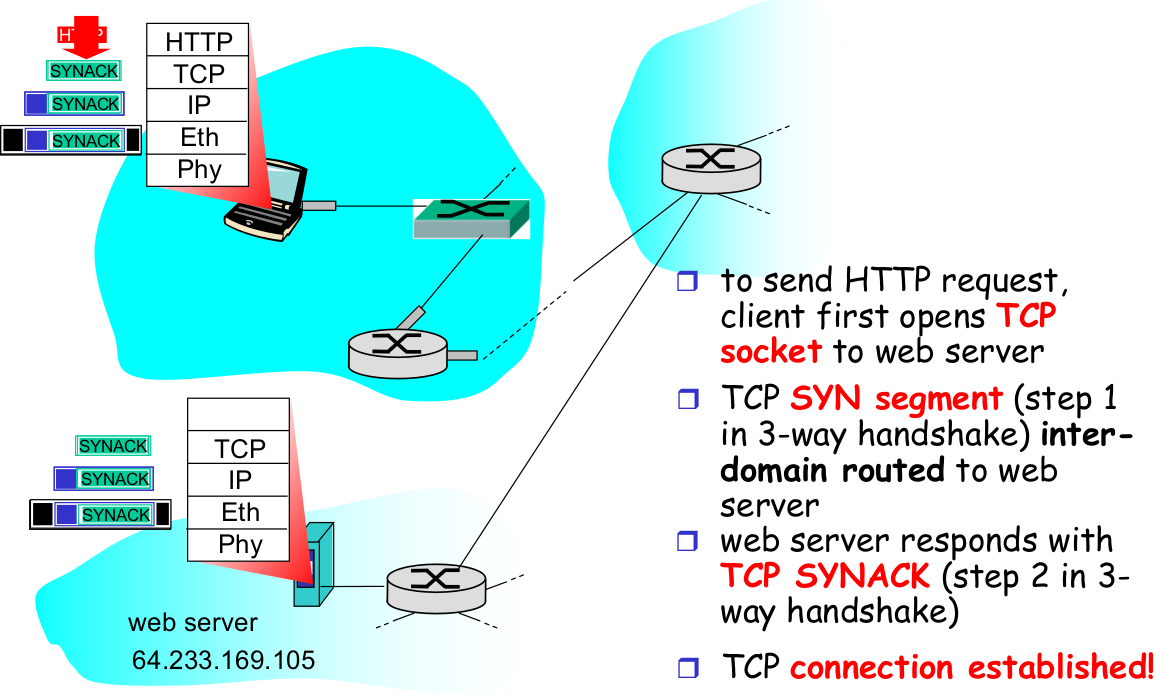
\includegraphics[width=0.48\textwidth]{day5}
  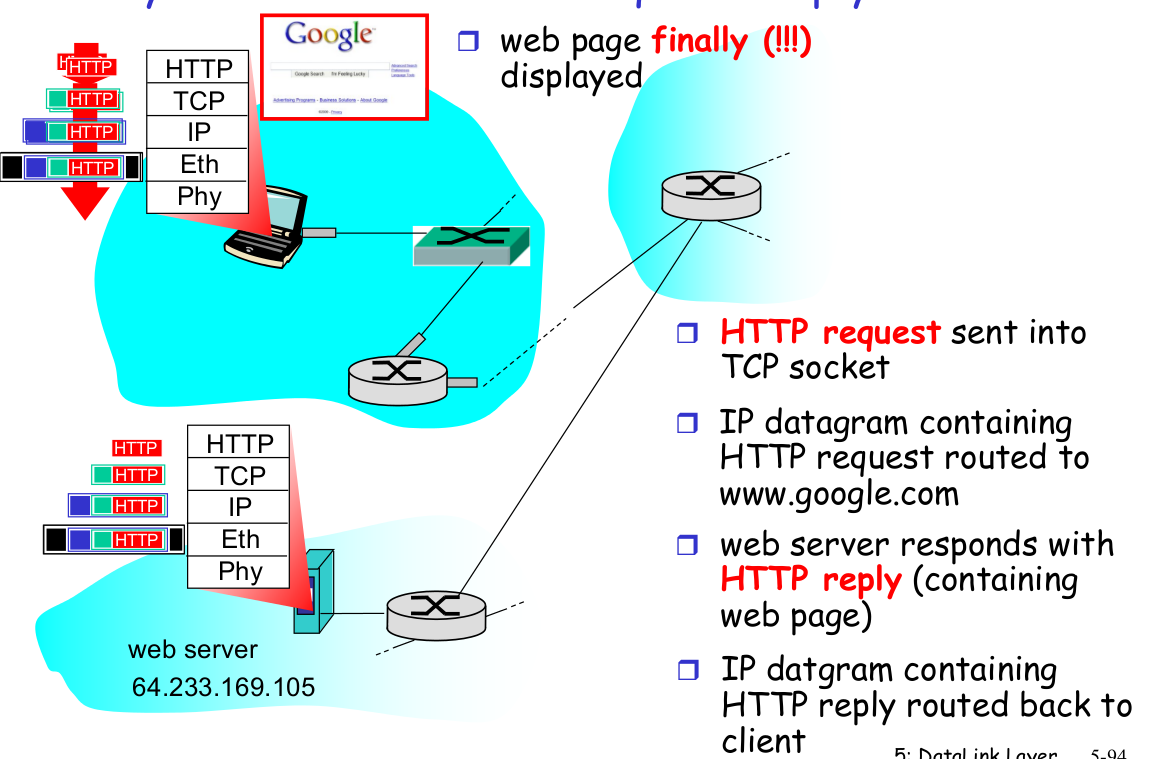
\includegraphics[width=0.48\textwidth]{day6}
\end{figure}
